\documentclass[11pt,a4paper]{article}
\usepackage{fontspec}
\setmainfont{NimbusRoman-Regular.otf}[Path=fonts/,BoldFont=NimbusRoman-Bold.otf,ItalicFont=NimbusRoman-Italic.otf,BoldItalicFont=NimbusRoman-BoldItalic.otf]
\usepackage[margin=24mm]{geometry}
\usepackage{amsmath,amssymb,booktabs,tabularx,graphicx,array,placeins}
\usepackage[colorlinks=true,allcolors=black]{hyperref}
\hypersetup{pdftitle={Source-Disjoint Evaluation Reveals Hidden Generalization Gaps in Literature-Derived Catalysis Machine Learning},
  pdfauthor={Zhang Junyu and Li Wenjie},
  pdfcreator={XeLaTeX}}
\setlength{\parskip}{2pt}
\emergencystretch=3em
\newcommand{\pp}{\,pp}
\newcommand{\mgg}{\,mg\,h$^{-1}$\,g$_{\mathrm{cat}}^{-1}$}

\title{\textbf{Source-Disjoint Evaluation Reveals Hidden Generalization Gaps\\
in Literature-Derived Catalysis Machine Learning:\\
Few-Label Adaptation, Input Representation,\\
and Reproducibility Audits}}
\author{Zhang Junyu\quad Li Wenjie\\[2pt]
\small College of Mechanical and Electronic Engineering,\\
\small China University of Petroleum (East China), Qingdao 266580, China}
\date{September 28, 2026}

\begin{document}
\maketitle

\begin{abstract}
Literature-derived catalytic datasets exhibit publication-level heterogeneity, requiring separate evaluation of unseen-source generalization and recovery using a few target-source labels.
We present a source-disjoint, label-budget-indexed, per-source-paired evaluation framework with negative controls across two reaction systems and four outcomes:
1,245 paired methanol conversion/selectivity records, 1,230 methanol space--time-yield (STY) records and 1,794 oxidative-coupling-of-methane (OCM) records.
Holding out entire leakage groups rather than random records reduces pooled $R^2$ by 0.20--0.47.
Five labels recover substantial error: in the core protocol, local ridge changes conversion source-equal MAE from 5.279 to 2.429\pp{}.
Paired representations and label permutations separate response level from true input--response correspondence; stronger local, residual and blend controls further isolate historical-response contributions.
At the same five-label budget and frozen blend, query-V acquisition changes STY MAE from 62.608 to 50.274 and composition-enriched OCM from 3.081 to 2.708\pp{}, reductions of 19.7\% and 12.1\% that pass the original five-panel family adjustment.
Applications cover 91 additional publication sources and one measured family of 1,739 records, in which composition acquisition improves nineteen of twenty identity-disjoint partitions.
Finally, author-protocol results from two open workflows can be recovered. Source-disjoint comparisons change Suvarna $R^2$ from 0.876 to 0.319, while the later matched-five-fold Xu audit changes source-equal MAE from 69.620 to 126.365 in native STY units.
The framework connects generalization gaps, label-assisted recovery, representation and measurement coverage with published-study reproducibility audits.
\end{abstract}

\section{Introduction}
Machine learning is increasingly used to accelerate the exploration of catalytic
composition--operating-condition spaces, and the training data for such models rarely come
from purpose-designed experiments. Instead, they are assembled from published literature:
individual papers report a handful of measurements, each produced with its own catalyst
preparation, characterization habits, feed purity, and reporting conventions. Curated
collections such as TheMeCat \cite{toldy}, the three-decade methanol synthesis
retrospective \cite{yan}, the Suvarna et al.\ space--time-yield dataset
\cite{suvarna}, and the Schmack et al.\ oxidative-coupling meta-analysis
\cite{schmack} have made this data mode practical, and models trained on such corpora
now routinely report high accuracy.

\paragraph{Two different generalization questions.} A random record-level split of a
literature-derived corpus answers a legitimate but specific question: how well does the
model interpolate to \emph{new records from the same sources it already saw}? Because
records from one publication share apparatus, catalyst family, and reporting practices,
random splits place near-duplicates of training records on the test side. The question
that matters for deployment --- \emph{how does the model behave on a literature source it
has never seen?} --- is answered instead by source-disjoint evaluation, in which entire
publications (or groups of records with identical upstream provenance) are held out.
Learning theory predicts that source-domain accuracy does not bound target-domain error
\cite{bendavid}, and grouped resampling is the standard remedy for clustered data
\cite{roberts}; what is missing in the catalysis setting is a quantified account of
the gap, across targets and reaction systems, together with an assessment of what can be
done about it.

\paragraph{Few-label adaptation as the practical response.} When a fitted model meets a
new literature source, the practitioner has a cheap middle option between trusting the
model and running a full campaign: collect a handful of labelled records from the new
source and adapt. Mean offsets, penalized affine corrections, empirical-Bayes shrinkage
\cite{efron}, and local regressors are classical tools for this; transfer of
multivariate calibration models has a long chemometric history \cite{feudale}. What
is missing is a budget-indexed, leak-controlled account: how much does each adapter buy
at $k$ labels, measured against strong simple baselines, with per-source pairing and
negative controls?

\paragraph{Diagnosing what adaptation exploits.} A mean offset can only repair a
source-level shift; a feature-dependent local model can also exploit within-source
label--input correspondence. These are different mechanisms with different implications,
and a paired bootstrap interval on average error does not distinguish them. We therefore
add label-permutation diagnostics, and we ask whether the input representation itself
limits what adaptation can find, using a strictly paired representation contrast on
identical records.

\paragraph{Published-study audits.} Finally, the phenomenon should not be an artifact of
our own benchmark. Two of the corpora we build on originate in published studies whose
data and code are public; we reproduce those workflows and apply the same
source-disjoint stress test to them.

\paragraph{Contributions.} This paper makes four contributions. (i)~An evaluation
framework for literature-derived catalysis data: source-disjoint outer folds over
leakage groups, label-blind fixed test sets, label budgets $k\in\{0,1,2,3,5,10\}$ with
nested calibration prefixes, strong simple adapters, per-source pairing, and negative
controls. (ii)~Quantified record-level optimism across two reaction systems and four
targets, together with zero-label behaviour and full few-label adaptation curves.
(iii)~A diagnosis of what few-label adaptation exploits --- source-level shifts versus
true label--input correspondence --- including a strictly paired representation
experiment showing that representation changes both the base model and the nature of the
adaptation gain. (iv)~Reproducibility audits of two open published workflows, separating
close reproduction from controlled split-design contrasts. The paper is a benchmark and
audit study; it proposes no new algorithm.

\section{Related work}
Grouped and blocked resampling designs for clustered data are standard
\cite{roberts}, and a recent catalysis benchmark compares formula-grouped with random
cross-validation \cite{wu}. Domain-adaptation theory separates source accuracy from
target error \cite{bendavid}. The adaptation estimators we evaluate are classical:
mean offsets and affine recalibration are standard practice \cite{steyerberg2019},
empirical-Bayes shrinkage goes back to Efron and Morris \cite{efron}, and
multivariate calibration transfer has been reviewed in chemometrics \cite{feudale}.
The curated datasets we build on are TheMeCat \cite{toldy}, the Communications
Engineering methanol retrospective \cite{yan}, the Schmack et al.\ OCM meta-analysis
\cite{schmack}, and the Suvarna et al.\ STY study \cite{suvarna}. None of these
sources reports source-disjoint evaluation with label budgets as its primary protocol;
positioning details are in Supplement A.

\section{Data}\label{sec:data}
\subsection{Data sources}
Table~\ref{tab:data} summarizes the corpora. All four targets come from two reaction
systems. The methanol corpus (1{,}245 paired records, 82 sources, 80 leakage groups)
provides CO$_2$ conversion and methanol selectivity in percentage points; it combines
TheMeCat v1 \cite{toldy} with the Communications Engineering retrospective dataset
\cite{yan}. The STY corpus (1{,}230 records, 109 sources) is derived from the
Suvarna et al.\ public dataset \cite{suvarna} under CC BY 4.0; twenty publication
identifiers overlap the conversion corpus, so the STY target is treated as a
same-reaction, different-target task, not an independent collection. The OCM corpus
(1{,}794 records, 408 sources, 405 leakage groups) comes from the Schmack et al.\\
meta-analysis \cite{schmack} and provides C$_2$ yield in percentage points. Targets
are never compared across units: percentage-point MAE for the three percent targets,
mg\,h$^{-1}$g$_{cat}^{-1}$ for STY.

\begin{table}[t]
\centering\small
\caption{Corpora, targets, and cohorts. ``Main cohort'' = sources whose calibration pool
supports the full $k\le10$ curve on a fixed test set of $\max(5,\lceil n/4\rceil)$
records.}
\label{tab:data}
\begin{tabularx}{\linewidth}{lXXXX}
\toprule
 & CO$_2$ conv. & MeOH sel. & MeOH STY & OCM C$_2$ yield \\\\
\midrule
Records & \multicolumn{2}{c}{1{,}245 (paired)} & 1{,}230 & 1{,}794 \\\\
Sources & \multicolumn{2}{c}{82} & 109 & 408 \\\\
Leakage groups & \multicolumn{2}{c}{80} & 109 & 405 \\\\
Main cohort & \multicolumn{2}{c}{32} & 28 & 22 \\\\
Units & \multicolumn{2}{c}{pp} & mg\,h$^{-1}$g$_{cat}^{-1}$ & pp \\\\
Feature families & \multicolumn{4}{l}{operating descriptors (+SBET for methanol;
+recorded composition for OCM F1)} \\\\
Licenses & \multicolumn{4}{l}{CC BY 4.0 (TheMeCat, OCM supplement, STY dataset)} \\\\
\bottomrule
\end{tabularx}
\end{table}

\subsection{Data reconstruction and inclusion criteria}
The methanol corpus is rebuilt row-by-row from the two upstream files (Table~\ref{tab:ledger}):
1{,}124 + 500 raw rows reduce to 748 + 497 admitted paired records after applying rules
fixed before any result was viewed --- both targets reported within $[0,100]$; temperature,
pressure, and H$_2$/CO$_2$ positive and reported; GHSV and BET allowed missing and imputed
within training folds; no performance-based filtering of any kind; genuine zero responses
retained; full-field upstream duplicates kept once, while records with identical conditions
and targets but different composition fields are retained as distinct measurements. Every
exclusion is logged row-by-row. Twenty records whose BET had been reconstructed as
$10^{\mathrm{LN}}$ in an early internal version are recomputed from the stored natural-log
field as $\exp(\mathrm{LN})$, with the correction logged. The OCM corpus applies the same
philosophy to the meta-analysis supplement (1{,}802 raw records over 412 publication
numbers; entries with missing or ambiguous references removed with a row-level log, and
three pairs of identical-citation sources merged).

\begin{table}[t]
\centering\small
\caption{Methanol corpus construction ledger. Excluded records are retained row-by-row in
an exclusion log; no performance-based filtering was applied.}
\label{tab:ledger}
\begin{tabular}{lrr}
\toprule
 & TheMeCat v1 & CommsEng MeOH \\\\
\midrule
Upstream file rows & 1{,}124 & 500 \\\\
Paired records admitted & 748 & 497 \\\\
No paired target & $-319$ & --- \\\\
Exactly one target missing & $-26$ & --- \\\\
Unresolved attribution / invalid DOI & $-30$ & $-3$ \\\\
Full-field upstream duplicates & $-1$ & --- \\\\
\bottomrule
\end{tabular}
\end{table}

\subsection{Source identity and leakage groups}
A source is a DOI-identifiable publication entry, not a laboratory: two papers from the
same group count as two sources, and one paper may span several catalysts. Conversely,
physical catalyst identity is not recovered across the historical corpus, so it does not establish new-family generalization; reported identifiers in the additional measured family are evaluated separately in Section 5.6. Records whose citations normalize to the same document,
or whose complete upstream measurements coincide, are merged into a leakage group; the
group is the atom of every outer split, so a group never straddles training and test
sides. OCM source numbers are the upstream meta-analysis's mapping rather than DOIs and
include some references and patents with non-uniform identifiers; this is carried as a
limitation.

\subsection{Unit harmonization and missingness}
Feature coverage for the methanol corpus: temperature 433--673~K, pressure 0.4--80 bar,
H$_2$/CO$_2$ 1--10, GHSV 0.87--240~L\,g$^{-1}$h$^{-1}$ (6.2\% missing), BET 2--975
m$^2$g$^{-1}$ (18.5\% missing); targets 0--59.6\% and 0--100\%. OCM: temperature
773--1223~K, CH$_4$ partial pressure 0.009--2.7 bar, O$_2$ 0.003--1.35 bar, CH$_4$/O$_2$
0.8--38.3, total pressure 0.11--4.5 bar, contact time 0.0017--182.5~s (2.5\% missing);
C$_2$ yield 0--37.0\%. STY: no missing features; STY 0.74--2620
mg\,h$^{-1}$g$_{cat}^{-1}$. All imputations are medians fitted on the current training
folds only. GHSV reference states and inert diluent definitions are not aligned
paper-by-paper; numerical agreement of GHSV therefore does not imply definitional
agreement, and this is preserved as a limitation rather than silently repaired.

\subsection{OCM F0/F1 representation pairing}
The OCM audit table records, for every modelled row, the catalyst identifier and
publication number of the upstream spreadsheet; joining the recorded composition onto
the modelled rows is an identity join (one-to-one on catalyst number and publication
number, zero unmatched rows, target values verified equal). F0 is the operating-only
representation (six descriptors). F1 adds the recorded catalyst composition: up to four
cation and two support slots, encoded role-separately with a reported indicator, the
known mol-fraction sum, a missing-amount count per species, and an explicit
unseen-species channel whose vocabulary is fitted on the current training partition only
(sodium is never treated as a missing marker; unlisted species are ``unreported'', not
provably absent). F0 and F1 share row identity, labels, sources, leakage groups, outer
folds, $T/U/A$ indices, calibration orders, and the model-selection procedure; the
contrast is therefore a strictly paired workflow comparison, not a causal composition
effect.


\subsection{Additional publication sources and a measured experimental family}
The extended evidence uses the same source-disjoint principle. After screening the full historical bibliography and removing three re-listed old sources,
the updated OCM compilation of Mine et al.\ \cite{mine} contributes 2,381 eligible measurements from 91 additional publication sources.
Fifty-two sources support complete random-query budget curves and forty support high-temperature queries.
Thermocatalytic eligibility, measured responses, consistent units and supported composition fields determine inclusion.
Historical preprocessing, predictors and hyperparameters are frozen before target support/query scoring.
Publication non-overlap is not evidence of independent laboratories.

A second application uses author-reported measurements from Nishimura et al.\ \cite{nishimura2023new}.
Stage eligibility, required response/temperature checks and duplicate catalyst--condition removal reduce 2,928 original rows to 1,739 measurements for 116 reported catalyst identifiers.
Five validation stages remain one publication and one experimental family. Four unavailable operating inputs and composition amounts retain the frozen missing-data treatment; physical values are not guessed.
In addition to ordinary queries, an initial identity holdout and twenty complete identity-disjoint partitions assign 29 identifiers to queries and 87 to the support pool.
Every record for an identifier remains on one side. Repetition measures query-composition sensitivity within this family.


\section{Evaluation protocol}\label{sec:protocol}
\begin{figure}[t]
\centering
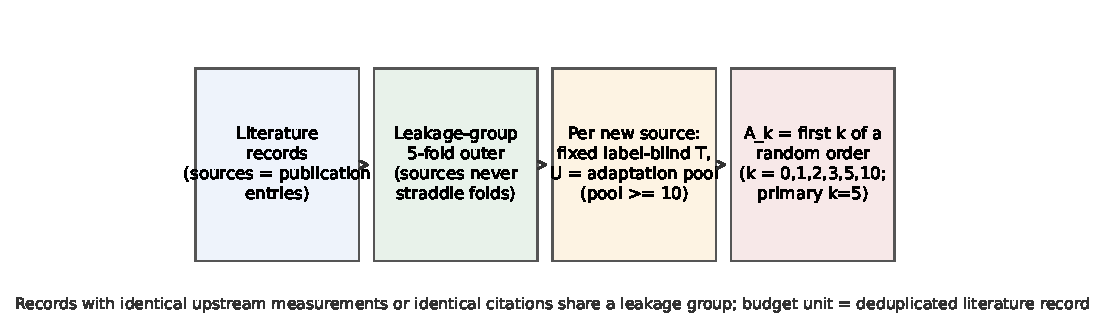
\includegraphics[width=\linewidth]{figs/fig1_design.pdf}
\caption{Evaluation design. Leakage groups are partitioned into five outer folds per
seed (five seeds); each group is tested exactly once per seed. Within a held-out source,
a fixed random split defines the label-blind test set $T$, and the remaining pool $U$ is
ordered randomly; $A_k$ is the first $k$ entries, with $A_1\subset A_2\subset A_3\subset
A_5\subset A_{10}$. Every adapter sees the same $T$, the same order, and the same fitted
base model.}
\label{fig:design}
\end{figure}
For each outer seed $s\in\{42,101,202,303,404\}$ the leakage groups are partitioned into
five folds; within each fold the base model (ridge over $\alpha\in\{0.1,1,10,100\}$ and
gradient-boosted trees over $n\in\{100,300\}\times$depth$\in\{2,3\}$ plus one deeper
configuration, selected by inner source-grouped cross-validation on inner equal-weight
MAE) is fitted on the training sources and predicts all held-out rows. Within each
held-out source, a label-blind fixed test set $T$ ($\max(5,\lceil n/4\rceil)$ records)
is scored, the remaining pool $U$ is ordered randomly, and $A_k$ is the first $k$
entries; fifty calibration orders are drawn per source. The primary budget is $k=5$;
$k=1$ and $k=10$ are designated secondary budgets. All adapters share the same $T$, the
same order, the same base prediction, and the same outer split; test-source information
never enters model selection, prior fitting, or imputation.

\paragraph{Adapters.} All adapters are strong simple baselines, not new algorithms. With
base prediction $p$, calibration labels $(y_A,p_A)$, and test predictions $p_T$: the
\emph{target mean/median} ignores the model; the \emph{mean offset} adds
$\overline{y_A-p_A}$, repairing the source-level residual mean; the \emph{penalized
affine} additionally allows a slope relationship between the residual and the centered
prediction, with the penalty fitted on training sources; \emph{empirical Bayes} shrinks
the observed offset toward a prior from training sources' out-of-fold residuals, which
protects single-label calibration; the \emph{local ridge} refits a ridge on $(x_A,y_A)$
with the training-side feature transform, exploiting within-source feature--label
correspondence. A temperature-only ridge is retained from the companion study.

\paragraph{Metrics.} The primary metric is source-equal MAE: per source, average the
absolute error over $T$ and over calibration repeats, then average equally across
sources. Row-weighted MAE and pooled $R^2$ (prediction-averaged unless stated) are
reported with explicit units; repeated calibration draws are never counted as independent
sources. Uncertainty is a leakage-group cluster bootstrap (100{,}000 draws, seed base
510{,}927), conditional on the fitted models --- an empirical between-source interval,
not a resampling of the full training procedure.

\paragraph{Negative controls.} Shuffled-label and shuffled-prediction controls are part
of the main protocol, and a dedicated alignment diagnostic (Section~\ref{sec:perm})
draws twenty uniform random permutations of each $A_k$'s labels, computing losses per
permutation before averaging. This is a retrospective diagnostic, not a formal
permutation test and not a deployment rule.


\paragraph{Extended predictors and historical response reuse.}
The strong simple controls are augmented with temperature-only ridge, residual ridge, shrinkage blending and historically tuned support-local radial-basis-function (RBF) regression.
Let $f_G$ denote the frozen historical predictor, $S$ the labelled support and $Q$ the query.
Local ridge fits $(z_S,y_S)$; residual ridge fits $y_S-f_G(S)$ and adds $f_G(Q)$.
For the same free-intercept linear fitting operator and regularization,
\begin{equation}\label{eq:ext_projection}
q_R(Q)-q_L(Q)=f_G(Q)-R_{S,\alpha}[f_G(S)](Q).
\end{equation}
This separates the historical response component not reconstructed by the support fit; matched-regularization ablations are retained separately.
The shrinkage blend $q_M=(1-w)q_L+wq_R$ selects $w$ using support leave-one-out evidence and historical pseudo-source priors, without query labels.
RBF and operating/composition block kernels are tuned on permitted historical data only. Full definitions and variants are given in Supplement B.

\paragraph{Equal-budget locations and representation crossing.}
Query-oriented V-optimal design greedily reduces working variance at the specified query inputs \cite{yubi,gorodetsky2016}.
Controls include random acquisition, coverage, pool-oriented V, kernel V and robust multi-view V; primary location comparisons fix the label budget and deployed predictor settings.
Each actual acquired support set is crossed with F0/F1 prediction, including a control that shuffles chemical row correspondence for acquisition alone.
The complete contrasts for learned source-contrast covariance, an adaptive view gate, block kernels, centered squared/absolute risk and covariance-averaged risk are retained.
They separate representation, predictor flexibility and acquisition effects rather than equating additional components with a performance contribution.

\paragraph{Prediction-operator risk and sensitivity.}
A fixed free-intercept kernel predictor has $\widehat y_Q=Ay_S$ and $A\mathbf1=\mathbf1$.
With working covariance $\Sigma_0$ and $B=[-A\ I]$, its squared risk is
$\mathcal R_0=|Q|^{-1}\operatorname{tr}(B\Sigma_0B^\top)$.
For $\|\Sigma-\Sigma_0\|_2\le\varepsilon$,
\begin{equation}\label{eq:ext_bound}
|\mathcal R_\Sigma-\mathcal R_0|\le
\varepsilon\left(1+\frac{\|A\|_F^2}{|Q|}\right).
\end{equation}
This explains support-noise amplification and query-task dependence. A covariance bound at an assumed radius is not a guarantee on actual MAE.
Derivations and penalty ablations are included in Supplement B.

\paragraph{Analysis layers and inference.}
The core benchmark and extended factorial analyses retain their own frozen historical fits, adapter parameters and support-order draws.
Unadapted or random-support point estimates can therefore differ slightly across analysis layers; every effect is computed against its matched within-layer control, never by cross-layer subtraction.
The core intervals retain their original inferential scope. The extended five-panel primary acquisition family uses adjusted intervals; other information interventions and opened-family analyses retain their exploratory/development status.
Publication sources, repeated seeds and catalyst partitions are reported separately.


\section{Results}\label{sec:results}
\subsection{Record-level versus source-disjoint evaluation (Research Question~1)}
\begin{figure}[t]
\centering
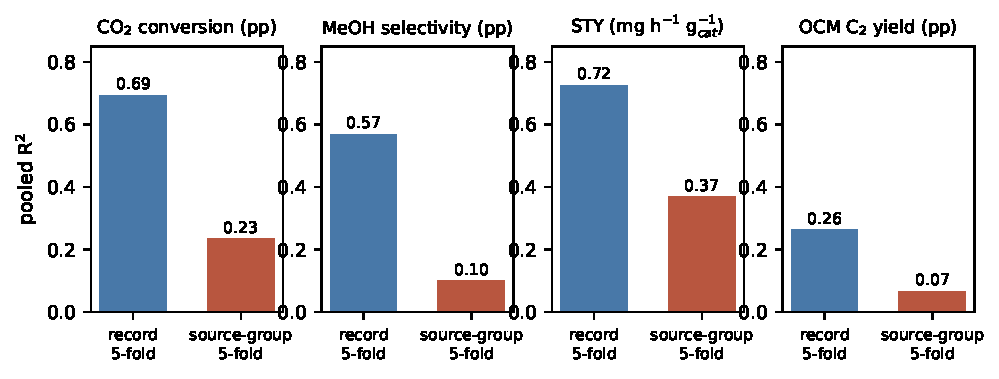
\includegraphics[width=\linewidth]{figs/fig2_split_contrast.pdf}
\caption{Record-level vs.\ source-group five-fold splits, fixed model and seeds; every
record is tested exactly once per seed in both modes. Pooled $R^2$ gaps: 0.460 (CO$_2$
conversion), 0.469 (selectivity), 0.356 (STY), 0.196 (OCM C$_2$ yield).}
\label{fig:split}
\end{figure}
With records, features, and the fixed model held identical, the split design dominates
every covariate choice we tested (Figure~\ref{fig:split}): pooled $R^2$ falls by 0.460
(CO$_2$ conversion), 0.469 (selectivity), 0.356 (STY), and 0.196 (OCM) when entire
leakage groups are held out instead of random records. The two designs answer different
generalization questions --- within-corpus interpolation versus new-source transfer ---
and we report the contrast descriptively; it is not a causal estimate of leakage. All
subsequent results use source-group splits.

\subsection{Zero-label behaviour and source shift (Research Question~2, start)}
On the all-source panel (held-out rows of all qualified sources, label-free methods
only), the base model's source-equal MAE beats the training-mean constant on every
target: 5.88 vs.\ 6.33\pp (conversion), 20.33 vs.\ 21.63\pp (selectivity), 5.47 vs.\\
5.82\pp (OCM), 136.6 vs.\ 187.2~\mgg{} (STY). Within the main adaptation cohorts the
ordering is panel-dependent: the base model wins on methanol conversion (5.279 vs.\\
5.910\pp) and STY (135.1 vs.\ 164.8~\mgg), but on OCM the training mean is slightly
better (5.177 vs.\ 5.285\pp) --- consistent with the representation limitation
quantified in Section~\ref{sec:repr}. Panels are never mixed.

\subsection{Few-label adaptation across budgets (Research Questions~2 and~3)}
\begin{figure}[t]
\centering
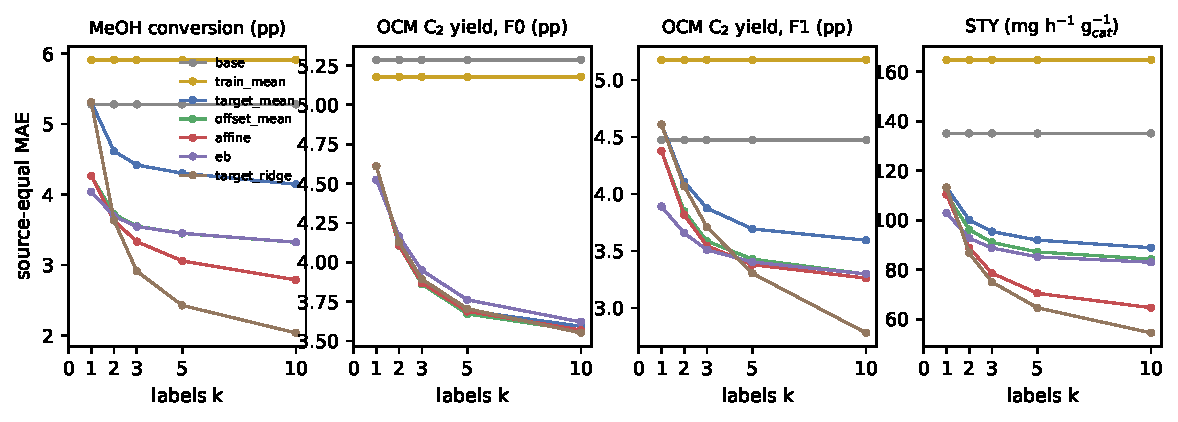
\includegraphics[width=\linewidth]{figs/fig3_learning_curves.pdf}
\caption{Main-cohort learning curves (random selector; source-equal MAE; $k=0$ from the
same fixed $T$). Units differ by panel and are never compared across panels.}
\label{fig:curves}
\end{figure}
\begin{table}[t]
\centering\small
\caption{Main cohort, primary budget $k=5$, random selector: source-equal MAE (unclipped
primary predictions) ; complete 95\% leakage-group bootstrap intervals are retained in Supplement A and the numerical registry. Units: pp for percent
targets; mg\,h$^{-1}$g$_{cat}^{-1}$ for STY.}
\label{tab:k5}
\begin{tabular}{lcccc}
\toprule
Method & Conv. (pp) & Sel. (pp) & OCM F0 (pp) & STY (mg/h/g) \\\\
\midrule
base (no labels) & 5.279 & 22.736 & 5.285 & 135.115 \\\\
train mean & 5.910 & 24.167 & 5.177 & 164.803 \\\\
target mean & 4.304 & 17.136 & 3.693 & 91.993 \\\\
target median & 4.443 & 18.100 & 3.817 & 92.259 \\\\
mean offset & 3.450 & 15.748 & 3.672 & 87.225 \\\\
affine & 3.060 & 12.540 & 3.688 & 70.508 \\\\
empirical Bayes & 3.452 & 15.990 & 3.762 & 85.244 \\
local ridge & \textbf{2.429} & \textbf{11.547} & 3.705 & \textbf{64.660} \\
\bottomrule
\end{tabular}
\end{table}
Table~\ref{tab:k5} and Figure~\ref{fig:curves} give the primary-budget results. Five
labels buy a large reduction, but the winning adapter differs by task. On methanol
conversion, the local ridge reduces base error by 54\% (5.28$\to$2.43\pp) and the affine
map reaches 3.06\pp; on STY the local ridge again dominates (64.7~\mgg{} vs.\ target-mean
92.0). On OCM-F0 every adapter lands within 0.15\pp of the target mean (3.67--3.82) and
the local ridge (3.705) does not beat the target mean (3.693). Per-source paired
contrasts (Table~\ref{tab:paired}) show that averages coexist with frequent per-source
harm: at $k{=}1$ the mean offset harms 15/32 (conversion) and 17/32 (selectivity)
sources, while EB shrinkage reduces the harmed counts to 11/32 on both targets without
raising the average. At $k{=}10$ the local ridge improves 32/32 and 29/32 sources
(conversion/selectivity). The three $R^2$ calibers and the full method set (fifteen
methods, both selectors, both budgets) are in the Supplementary Material.

\begin{table}[t]
\centering\small
\caption{Main-cohort per-source paired contrasts: mean MAE difference (method $-$
reference, pp) and improved sources out of 32 at $k=1,5,10$ (random selector).
Negative differences favour the method.}
\label{tab:paired}
\begin{tabular}{llrrr}
\toprule
Target & Comparison & $k=1$ & $k=5$ & $k=10$ \\
\midrule
CO$_2$ conversion & EB vs.\ base & $-1.24$ (21/32) & $-1.83$ (23/32) & $-1.95$ (24/32) \\
 & affine vs.\ mean offset & 0 (constr.) & $-0.39$ (25/32) & $-0.53$ (24/32) \\
 & local ridge vs.\ EB & $+1.27$ (8/32) & $-1.02$ (25/32) & $-1.29$ (28/32) \\
\midrule
Methanol selectivity & EB vs.\ base & $-3.87$ (21/32) & $-6.75$ (20/32) & $-7.20$ (20/32) \\
 & affine vs.\ mean offset & 0 (constr.) & $-3.21$ (22/32) & $-3.89$ (22/32) \\
 & local ridge vs.\ EB & $+2.35$ (7/32) & $-4.44$ (21/32) & $-5.49$ (23/32) \\
\bottomrule
\end{tabular}
\end{table}


\subsubsection{Stronger controls: response level, local relations and historical response}
Table~\ref{tab:ext_information} extends the predictor comparison to nine strategies and includes OCM F1.
Within this matched extended protocol, F1 source-equal MAE falls from 4.527 for the unadapted predictor to 3.693 for the support mean, 3.374 for local ridge, 3.109 for residual ridge and 3.081\pp{} for blending.
The corresponding STY global, support-mean, local-ridge and blend errors are 139.258, 91.993, 65.210 and 62.608\mgg{}.
This extends the original budget-curve finding: few target responses reveal both a source level and useful input--response relations.
The incremental contribution of historical responses must be compared against local fits using the same labels.
\begin{table}[htbp]\centering\footnotesize
\setlength{\tabcolsep}{4pt}
\caption{Extended information controls with five random support labels. Each panel shares support/query records. Frozen fits and support orders belong to this analysis layer, separately from the core benchmark in Table~\ref{tab:k5}; gains are not computed across tables. STY uses native units; other responses use percentage points.}\label{tab:ext_information}
\begin{tabular}{lrrrrr}
\toprule
Strategy & Conv. & Sel. & OCM F0 & OCM F1 & STY \\
\midrule
Global & 5.271 & 22.740 & 5.302 & 4.527 & 139.258 \\
Support mean & 4.304 & 17.136 & 3.693 & 3.693 & 91.993 \\
Offset & 3.455 & 15.747 & 3.672 & 3.423 & 88.265 \\
Affine & 3.083 & 12.539 & 3.694 & 3.360 & 71.225 \\
EB offset & 3.457 & 15.988 & 3.759 & 3.415 & 86.510 \\
Local ridge & 2.429 & 11.547 & 3.655 & 3.374 & 65.210 \\
Temperature ridge & 2.519 & 11.535 & 3.677 & 3.677 & 87.098 \\
Residual ridge & 2.720 & 12.077 & 3.701 & 3.109 & 69.889 \\
Shrinkage blend & 2.441 & 11.584 & 3.660 & 3.081 & 62.608 \\
\bottomrule
\end{tabular}

\end{table}

\subsubsection{Additional-source application and equal-budget measurement locations}
Across the 52 additional publication sources eligible for complete curves, F1 five-label random-query MAEs are 6.120, 4.490, 3.593 and 3.552\pp{} for global, support mean, local ridge and blending, respectively (Table~\ref{tab:ext_external}).
The forty-source high-temperature population is reported separately in the same table.
These observations extend the value of label-assisted conditional calibration; publication counts do not establish laboratory independence.
\begin{table}[htbp]\centering\footnotesize
\setlength{\tabcolsep}{4pt}
\caption{Frozen five-label application on additional publication sources: 52 random-query and 40 high-temperature sources. F0/F1 are paired views of the same records. MAE is in percentage points.}\label{tab:ext_external}
\begin{tabular}{lrrrr}
\toprule
Strategy & F0 random & F1 random & F0 high T & F1 high T \\
\midrule
Global & 5.973 & 6.120 & 5.699 & 5.140 \\
Support mean & 4.490 & 4.490 & 5.556 & 5.556 \\
Offset & 4.502 & 4.606 & 5.512 & 5.397 \\
Affine & 4.284 & 4.410 & 5.209 & 5.328 \\
EB offset & 4.545 & 4.621 & 5.205 & 4.942 \\
Local ridge & 4.045 & 3.593 & 4.801 & 4.365 \\
Temperature ridge & 3.779 & 3.779 & 4.697 & 4.697 \\
Residual ridge & 4.421 & 3.716 & 5.375 & 4.454 \\
Shrinkage blend & 4.054 & 3.552 & 4.806 & 4.335 \\
\bottomrule
\end{tabular}

\end{table}

At the same label budget and frozen blend, query V changes STY MAE from 62.608 to 50.274\mgg{} and OCM F1 from 3.081 to 2.708\pp{}, corresponding to point reductions of 19.7\% and 12.1\% (Table~\ref{tab:ext_acquisition}).
Both pass adjustment within the original five-panel acquisition family.
Thus locations, as well as the number of labels, influence the use of a fixed measurement budget. All other panels remain visible.
\begin{table}[htbp]\centering\footnotesize
\setlength{\tabcolsep}{4pt}
\caption{Query V versus random supports at five labels with the same frozen blend. Source counts are panel-specific. Adjusted intervals concern native-unit MAE differences, not ratios of errors.}\label{tab:ext_acquisition}
\begin{tabular}{lrrrrl}\toprule Panel & $n$ & Random & Query V & Gain (\%) & Adjusted $\Delta$ interval\\\midrule
Conversion & 32 & 2.441 & 2.121 & 13.1 & [-0.707, 0.068]\\
Selectivity & 32 & 11.584 & 10.683 & 7.8 & [-2.140, 0.615]\\
STY & 28 & 62.608 & 50.274 & 19.7 & [-25.965, -2.874]\\
OCM F0 & 22 & 3.660 & 3.768 & -3.0 & [-0.355, 0.714]\\
OCM F1 & 22 & 3.081 & 2.708 & 12.1 & [-0.746, -0.056]\\
\bottomrule\end{tabular}

\end{table}
\begin{figure}[htbp]\centering
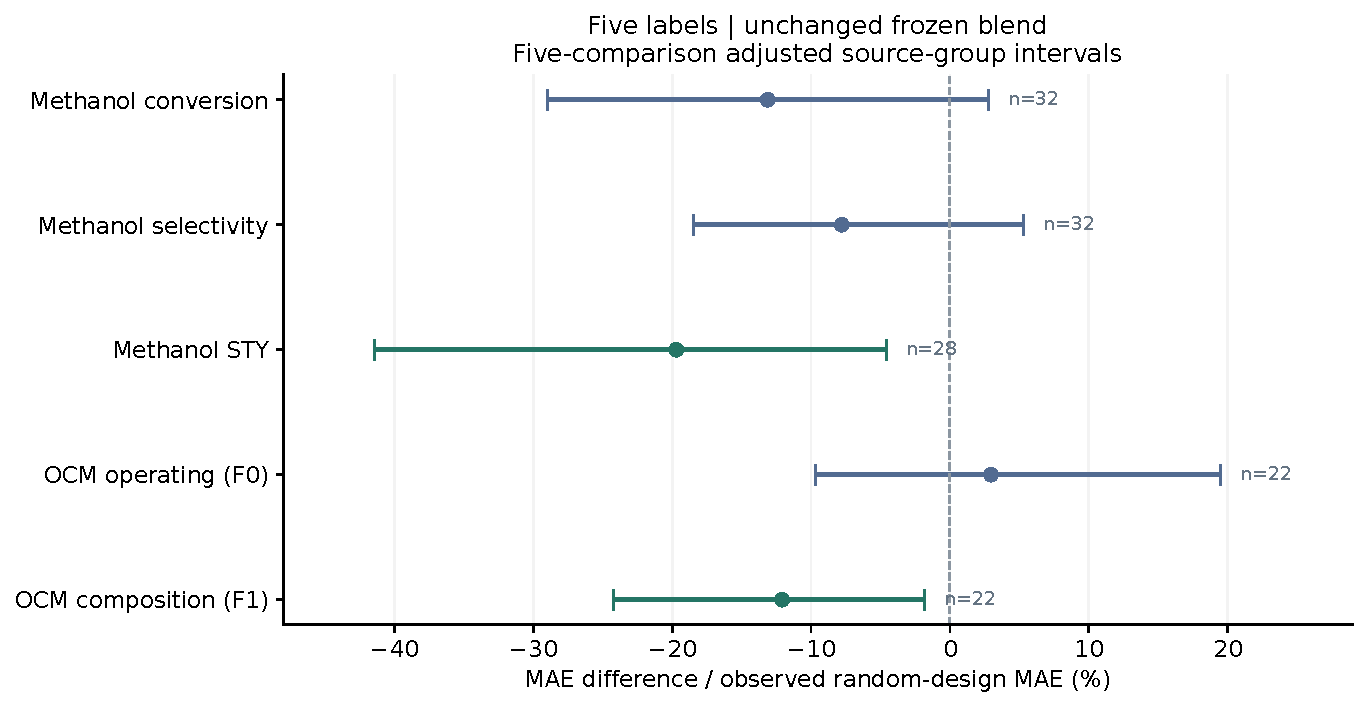
\includegraphics[width=\linewidth]{figs/extension_acquisition.pdf}
\caption{Matched acquisition effects across five panels. Native-unit adjusted difference intervals are divided by each fixed random MAE for display; response units are not pooled.}\label{fig:ext_acquisition}
\end{figure}

On the author-measured family's fixed ordinary query, the same composition-V supports give F1 errors of 5.869 for global, 5.959 for the support mean, 4.170 for local ridge, 4.213 for blending and 3.813\pp{} for the historically tuned local RBF.
Composition V changes blend MAE from the matched random value 4.787 to 4.213, a 12.0\% point reduction.
These observations distinguish local conditional relations from a source level and motivate the stronger nonlinear local control.


\subsection{Representation changes both prediction and adaptation
(Research Question~4)}
\label{sec:repr}
Representation variation is large in the OCM corpus: nine of the twenty-two main-cohort
sources have a single unique F0 operating vector, and 391 of 505 F0 records share their
complete six-feature vector with a same-source record of different outcome; adding the
recorded composition (F1) removes all constant sources and reduces collisions to 36
records (all-source counts: 303$\to$168). The paired results
(Figure~\ref{fig:f0f1}) are consistent with the representation mattering: base MAE
improves by 0.811\pp ($5.285\to4.474$; CI $[-1.490,-0.189]$), affine by 0.309\pp
(CI $[-0.573,-0.063]$), and local ridge by 0.402\pp at $k=5$ (CI $[-0.601,-0.228]$)
and 0.772\pp at $k=10$ (CI $[-1.144,-0.434]$). Because both arms share the
model-selection procedure, this is a workflow-level association; no composition-causal improvement is established. Even with F1, calibrated errors ($\approx3.3\pp$) remain well below the F1
base error (4.47\pp): the richer representation is associated with better base-model accuracy, and calibration still helps on top.

\begin{figure}[t]
\centering
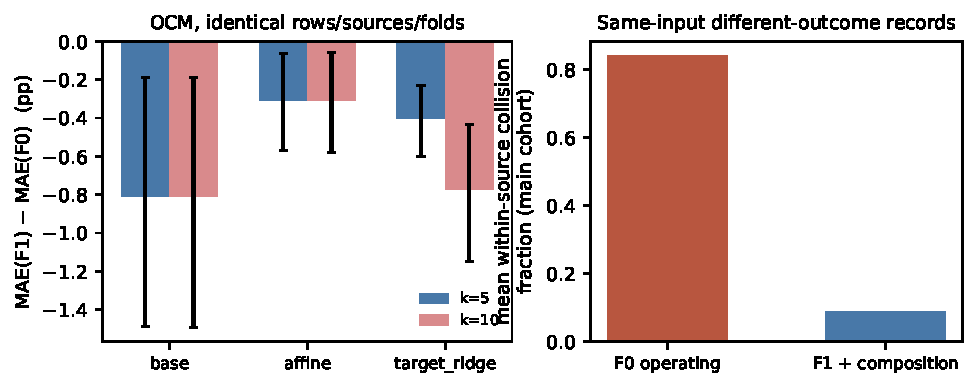
\includegraphics[width=\linewidth]{figs/fig4_f0_f1_paired.pdf}
\caption{Left: OCM F1$-$F0 paired contrasts (source-equal MAE, negative = composition
associated with improvement) at $k=5$ and $k=10$. Right: mean within-source fraction of
records whose complete input vector is shared with another same-source record of
different outcome (main cohort); such rows are retained --- they may be genuine
replicates or carry unrecorded conditions.}
\label{fig:f0f1}
\end{figure}


\subsubsection{Chemistry can also determine where to measure}
In the matched crossing over 22 historical OCM sources, composition V changes frozen F0 blend MAE from its matched random value 3.705 to 3.370\pp{}, although that predictor never receives composition.
Shuffling chemical row correspondence for acquisition alone raises MAE to 3.647.
For F1, the composition-V and shuffled results are 2.708 and 3.039\pp{}, respectively.
Each support set is shared across F0/F1 prediction, locating this information value in acquisition rather than only in additional prediction inputs.
This crossing retains its own random support orders; its F0 random value is not subtracted from baselines in other analysis layers.
\begin{figure}[htbp]\centering
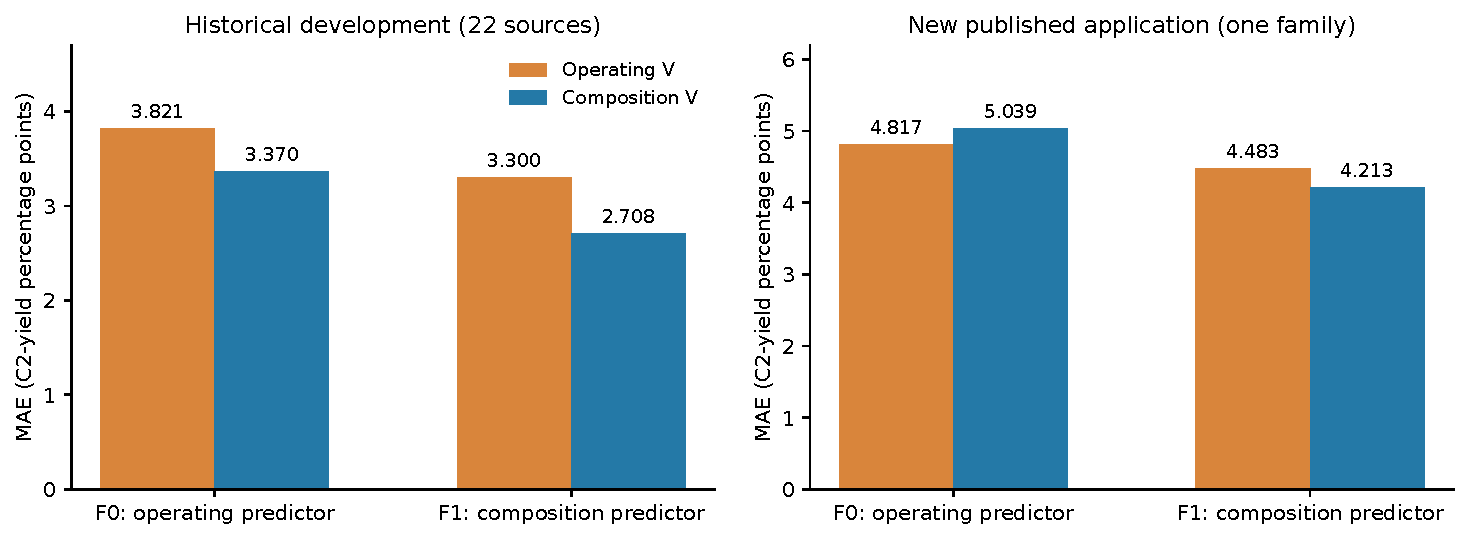
\includegraphics[width=\linewidth]{figs/extension_crossing.pdf}
\caption{Acquisition--prediction representation crossing. Historical and author-measured applications are reported separately; every acquired support set is shared across F0/F1 prediction. The useful acquisition view depends on predictor and source.}\label{fig:ext_crossing}
\end{figure}

On the author-measured family, operating V outperforms composition V for F0 (4.817 versus 5.039\pp{}), while F1 benefits more from composition V.
The original representation comparison therefore extends to two testable roles: chemical descriptors can support response fitting and measurement allocation, with the useful view determined by the deployment task.


\subsection{What does few-label adaptation exploit? (Research Question~3)}\label{sec:perm}
\begin{figure}[t]
\centering
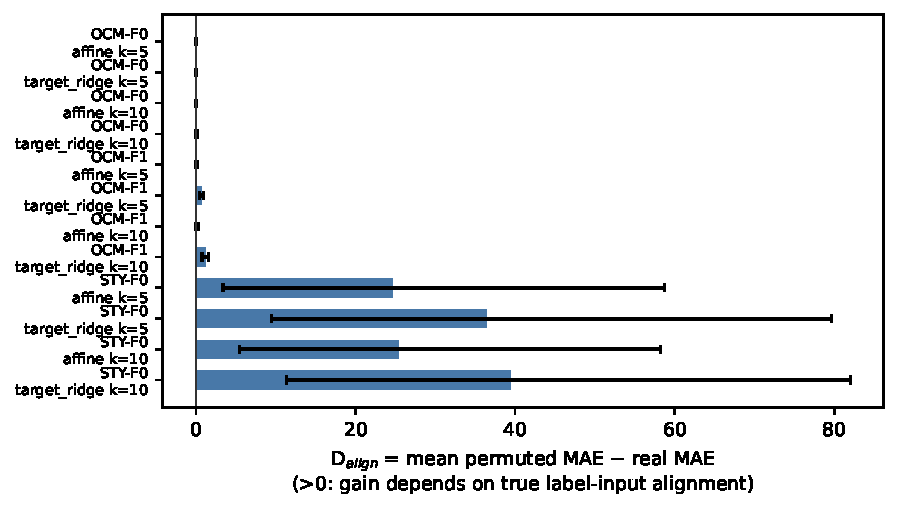
\includegraphics[width=.86\linewidth]{figs/fig5_permutation.pdf}
\caption{Alignment diagnostic on the main cohort (allocation 0, repeats 0--19, twenty
uniform label permutations per $A_k$ shared between affine and local ridge; losses
averaged per permutation first). Positive $D_{\mathrm{align}}$: the method's gain
depends on the true label--input correspondence. $k=1$ has no non-trivial permutation
(not applicable).}
\label{fig:perm}
\end{figure}
Figure~\ref{fig:perm} separates level-dominated from alignment-dependent gains. On
OCM-F0, $D_{\mathrm{align}}$ for the affine map is 0.015 (CI $[-0.001,0.042]$): the gain
survives label permutation, consistent with the degeneracy mechanism --- when the
source representation is constant, slope-dependent corrections reduce to a function of
the selected labels' mean level, and the result is invariant to permutation
\emph{within the same selected label set}, though not necessarily to drawing a different
label set. On OCM-F1 the affine diagnostic stays near zero, but the local-ridge
diagnostic is strongly positive ($0.66\pp$ at $k=5$, CI $[0.44,0.90]$; $1.14\pp$ at
$k=10$): once composition makes the inputs informative, the local ridge exploits true
label--input correspondence. On STY both methods are alignment-dependent (24.6 and
36.5~\mgg{} at $k=5$).


\subsubsection{Correspondence and historical-response controls for the frozen blend}
For five-label query-V supports, the extended intervention preserves the label multiset and mean but changes OCM F1 blend MAE from 2.708 to 3.548\pp{}.
The difference is 0.840 with an exploratory conditional 95\% interval [0.478, 1.237].
Differences for conversion, selectivity and STY are 2.015, 6.040 and 30.671 native units; OCM F0 changes by only 0.047\pp{} with an interval spanning zero (Table~\ref{tab:ext_alignment}).
These observations complement the original local-ridge diagnostic without pooling effects from different predictors or support rules.
\begin{table}[htbp]\centering\footnotesize
\setlength{\tabcolsep}{4pt}
\caption{Extended permutation diagnostic for five-label query-V supports. Each arm retains the same support set. Intervals are exploratory conditional 95\% grouped-bootstrap intervals, not a redefined family-adjusted primary comparison.}\label{tab:ext_alignment}
\begin{tabular}{lrrrl}\toprule
Panel & Aligned & Permuted & $\Delta$ MAE & 95\% interval \\ \midrule
Conversion & 2.121 & 4.135 & 2.015 & [1.253, 2.851] \\
Selectivity & 10.683 & 16.723 & 6.040 & [3.693, 8.513] \\
STY & 50.274 & 80.945 & 30.671 & [10.436, 59.603] \\
OCM F0 & 3.768 & 3.815 & 0.047 & [-0.009, 0.134] \\
OCM F1 & 2.708 & 3.548 & 0.840 & [0.478, 1.237] \\
\bottomrule\end{tabular}

\end{table}

Equation~\ref{eq:ext_projection} further separates local fitting from historical-response reuse.
F1 residual and blend point estimates improve on local ridge, but matched-regularization historical-component intervals span zero in each panel.
The positive supported conclusion is identifiable response-level and correspondence information in target labels; the additional value of historical responses is estimated task by task against strong local controls.
Permuting observed labels does not identify the physical causal effect of a chemical component.


\subsection{T-allocation sensitivity, ranking stability, and the small-source panel
(Research Question~5)}
\begin{figure}[t]
\centering
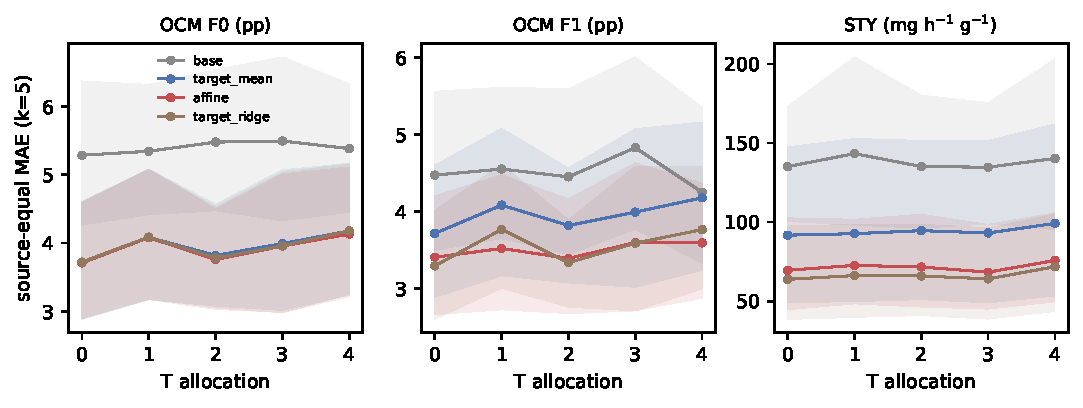
\includegraphics[width=\linewidth]{figs/fig6_allocation.pdf}
\caption{$T$-allocation sensitivity at $k=5$ (main cohort; allocation 0 is the fixed
design used everywhere else; allocations 1--4 are independent frozen allocations).}
\label{fig:alloc}
\end{figure}
Repeating the fixed-$T$ construction under four additional frozen allocations
(Figure~\ref{fig:alloc}) moves main-cohort MAE by at most $\approx0.4\pp$ (OCM) and
$\approx8$~\mgg{} (STY) at $k=5$. Method rankings are two-sided stable --- base and
train mean occupy the last two positions in every allocation on every task, and STY's
top pair (local ridge, then affine) is rank-stable --- but not universally invariant:
OCM-F1's local ridge ranks 1--4 across allocations, so its relative ranking against affine and empirical Bayes depends on the allocation; no allocation-averaged advantage is claimed. Per-source outcomes are heterogeneous: at $k=5$ the
affine-versus-offset contrast improves 25/22 (conv./sel.), 8 (OCM-F0), 16 (OCM-F1), and
23 (STY) sources; harms 6/9, 5, 6, and 5; the remaining are numerical ties. The independent small-source panel
(calibration pool 3--9 records: methanol 22, OCM 45, STY 43 sources) shows the same
qualitative picture at $k=3$ (Supplementary Material); it never enters main-cohort
numbers.


\subsubsection{Measurement coverage under catalyst-identity shift}
Extending the original allocation sensitivity to catalyst identity, the initial holdout gives strong-local-RBF five-label MAE 3.689\pp{} for expanded-kernel-risk acquisition versus matched random 4.818 and composition V 4.680.
On the same family's ordinary query, the corresponding errors are 5.145, 4.792 and 3.813.
Each query task retains its own random control: acquisition rankings can change with the identities to be predicted.

Across twenty identity-disjoint partitions, composition V changes mean RBF MAE from 4.922 to 4.107\pp{}, a 16.6\% reduction computed as the ratio of mean errors, improving nineteen partitions (Table~\ref{tab:ext_repeated}).
Pool V, expanded-kernel risk and RBF-matched risk improve eighteen, fifteen and thirteen partitions, respectively.
The positive result is useful chemistry-guided coverage at the same budget for identity-disjoint queries in this family.
Shared measurements and a shared experimental family mean that twenty partitions are not twenty independent sources or a 95\% future success probability.
\begin{table}[htbp]\centering\footnotesize
\setlength{\tabcolsep}{4pt}
\caption{Twenty complete catalyst-identity-disjoint partitions within one opened measured family, using five labels and the same fixed historical-selected RBF. Differences are method minus matched random within partition, in percentage points. Ranges describe partition scatter, not cross-source confidence intervals.}\label{tab:ext_repeated}
\begin{tabular}{lrrll}\toprule
Acquisition & Mean MAE & Mean $\Delta$ & Partition $\Delta$ range & Improved \\ \midrule
Random & 4.922 & +0.000 & +0.000 to +0.000 & 0/20 \\
Composition V & 4.107 & -0.815 & -1.616 to +0.120 & 19/20 \\
Operating V & 4.926 & +0.004 & -1.025 to +0.731 & 11/20 \\
Pool V & 4.221 & -0.701 & -1.272 to +0.210 & 18/20 \\
Expanded-kernel risk & 4.480 & -0.441 & -1.545 to +0.498 & 15/20 \\
RBF-matched risk & 4.652 & -0.270 & -1.360 to +0.621 & 13/20 \\
Penalized RBF risk & 4.652 & -0.270 & -1.360 to +0.621 & 13/20 \\
\bottomrule\end{tabular}

\end{table}
\begin{figure}[htbp]\centering
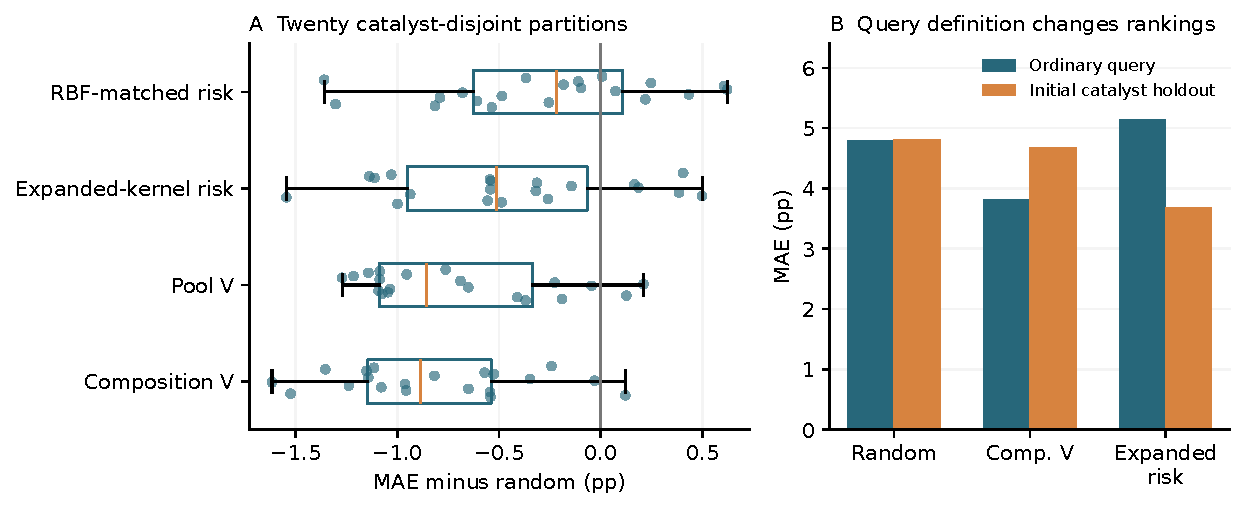
\includegraphics[width=\linewidth]{figs/extension_sensitivity.pdf}
\caption{Query task and measurement coverage. A retains every paired difference across twenty partitions; B retains the separate matched ordinary-query and initial identity-holdout comparisons. The tasks do not share a common random baseline.}\label{fig:ext_sensitivity}
\end{figure}

\subsubsection{Complete flexibility and risk-objective controls}
Across the 22 historical sources, fixed-strong-RBF five-label MAEs are 3.288 for random, 2.851 for composition V, 2.784 for expanded-kernel risk, 2.828 for RBF-matched risk and 2.913\pp{} for penalized RBF risk (Table~\ref{tab:ext_risk}).
The median within-source rank correlation between working risk and actual MSE is 0.514: the risk is informative but not calibrated in outcome units.
Penalty tuning selects zero in 23 of 25 historical outer fits and 0.1 in two; the full-history choice is zero.
Equation~\ref{eq:ext_bound} therefore explains sensitivity without establishing a universally superior penalty.
\begin{table}[htbp]\centering\footnotesize
\setlength{\tabcolsep}{4pt}
\caption{Fixed-strong-RBF historical random-query F1 comparison: five labels and 22 sources. Working risk is a dimensionless proxy, not actual MAE in percentage points.}\label{tab:ext_risk}
\begin{tabular}{lrrr}\toprule
Acquisition & MAE (pp) & Working risk & Amplification \\ \midrule
Random & 3.288 & 0.137 & 0.563 \\
Composition V & 2.851 & 0.091 & 0.583 \\
Expanded-kernel risk & 2.784 & 0.090 & 0.627 \\
RBF-matched risk & 2.828 & 0.090 & 0.664 \\
Penalized RBF risk & 2.913 & 0.091 & 0.653 \\
\bottomrule\end{tabular}

\end{table}

Supplement B also retains the development controls: learned source-contrast prediction with linear query V gives historical MAE 3.034\pp{} (3.287 with contrast V), versus 2.708 for frozen blending;
the adaptive view gate gives 3.373 versus fixed composition V 3.370 and retains composition in 109 of 110 primary source--seed episodes.
The covariance-averaged absolute-risk candidate does not pass its five family-adjusted superiority contrasts.
The full same-tuning block/isotropic-kernel, finite-intercept/centered-risk, squared/absolute-risk and frozen/retuned-policy matrices are preserved.
The contribution is reproducible equal-budget utility and its conditions, rather than additional components alone.


\subsection{Reproducibility audits of two published studies (Research Question~6)}
\label{sec:audit}
The stress tests above act on our own benchmark. The natural final question is external:
what happens when the same stress test is applied to published studies whose data and
code are public? We select two methanol-STY studies with complete public assets for
direct comparability \cite{suvarna,xu}. All assets --- repositories,
commits, dataset hashes --- are archived in the reproduction package. We use no
accusatory language: what is audited is the extrapolation scope of an evaluation design,
not the credibility of the authors. Reproduction classes are stated uniformly: the
Suvarna case is a close reproduction (its notebook input file is not public; four
documented compatibility fixes on the published dataset), and the Xu case is an
original-flow reproduction (the author's code ran unmodified).

\textbf{Case 1: Suvarna et al.\ (2022, Appl.\ Catal.\ B).} The author repository
(MIT, commit \texttt{0dac9383}) contains the published dataset (1{,}234 rows, every row
with a Reference DOI, zero unmapped) and the author's notebook with committed outputs:
random 80/20 (seed 22), cv=3 grid search on train, three model families. Tier A applies the
published workflow with a compatibility reconstruction on the full public dataset
before the split; it is used only to establish close reproduction of the
published random-split protocol, not as a leakage-controlled comparison. The
re-run gives XGB test $R^2$ 0.9210 versus the author's
committed 0.9132 (gap $+0.008$; RF/GBT $-0.007/+0.012$) --- a close reproduction. The
strictly controlled contrast holds rows, features, and configurations fixed and varies
only the split: in matched five-fold designs, XGB source-equal MAE rises from 57.9
(record-level) to 124.0 (source-disjoint) and the stacked pooled $R^2$ (the predeclared
primary caliber) falls from 0.876 to 0.319.

\textbf{Representation, strictly paired.} On the same 1{,}234 rows and the same folds,
F5 (operating-only: temperature, pressure, H$_2$/CO$_2$, GHSV, SBET --- no categorical
columns) versus F17 (all published descriptors), with per-source paired deltas and
DOI-cluster bootstrap, gives: under record-level splits F17 is significantly better for
all three models (XGB $-12.15$ [$-16.63,-7.42$]); under source-disjoint evaluation the GBT and RF differences are inconclusive (GBT $-0.05$ [$-13.45,+16.73$]; RF $+2.90$ [$-8.72,+15.42$]; CIs cross zero) and only XGB retains a clear advantage ($-29.56$ [$-42.68,-17.05$]; negative = richer descriptors better).The benefit of the
richer descriptors is therefore model-dependent, and even where it exists,
source-disjoint performance remains well below record-level performance; composition
does not close the source shift.

\textbf{Case 2: Xu et al.\ (2026, npj Comput. Mater.).}
The author repository (commit \texttt{b7291de8}) contains 1,839 records and complete prediction code.
The original-flow A reproduction gives CatBoost test $R^2$ 0.8911 (CV $0.8887\pm0.0121$).
The source audit uses 1,757 DOI-known rows and 156 canonical sources; 82 DOI-missing records are not treated as one real source.
The archived fixed-configuration B results retain their split labels: log1p $R^2$ is 0.896 for random 80/20 and 0.251 for source five-fold evaluation.
A later strictly matched audit fixes the same five seeds, record set and XGBoost 3.2.0 configuration (500 trees, depth 6, learning rate .05, random state 42) for record and DOI-source five-fold fits.
Pooling record errors within each source/seed before averaging sources gives corrected native-STY MAEs of 69.6198 and 126.3649, replacing the earlier five-fold weighting claim.
The response is fitted in log1p space and inverse-transformed for native-unit MAE.
Category maps, medians and scaling use training records only, and DOI is not a predictor.
Archived random-80/20 source-equal MAE is separately 62.9776 and is not a full-five-fold baseline.
The original nested/frozen-author-parameter C/D layers and the pandas-dependent category-detection difference remain documented in Supplement A.

\begin{table}[t]\centering\small
\caption{Author-flow reproduction and source-disjoint audits. A reproduces each author protocol; matched comparisons retain the same records, settings and split seeds. MAE is native STY and $R^2$ spaces are identified separately.}\label{tab:audit}
\begin{tabularx}{\linewidth}{lXXX}\toprule
Study & Author-flow reproduction & Source-disjoint comparison & Comparison scope\\\midrule
Suvarna 2022 & XGB $R^2$ 0.9210 vs.\ author 0.9132; close reproduction & MAE 57.9$\to$124.0; $R^2$ 0.876$\to$0.319 & Matched five-fold, native STY\\
Xu 2026 & CatBoost $R^2$ 0.8911; original-flow reproduction & Corrected MAE 69.620$\to$126.365 & Same five folds/seeds, XGB 3.2.0; log1p fit, native-unit MAE\\
\bottomrule\end{tabularx}\end{table}


\begin{figure}[t]
\centering
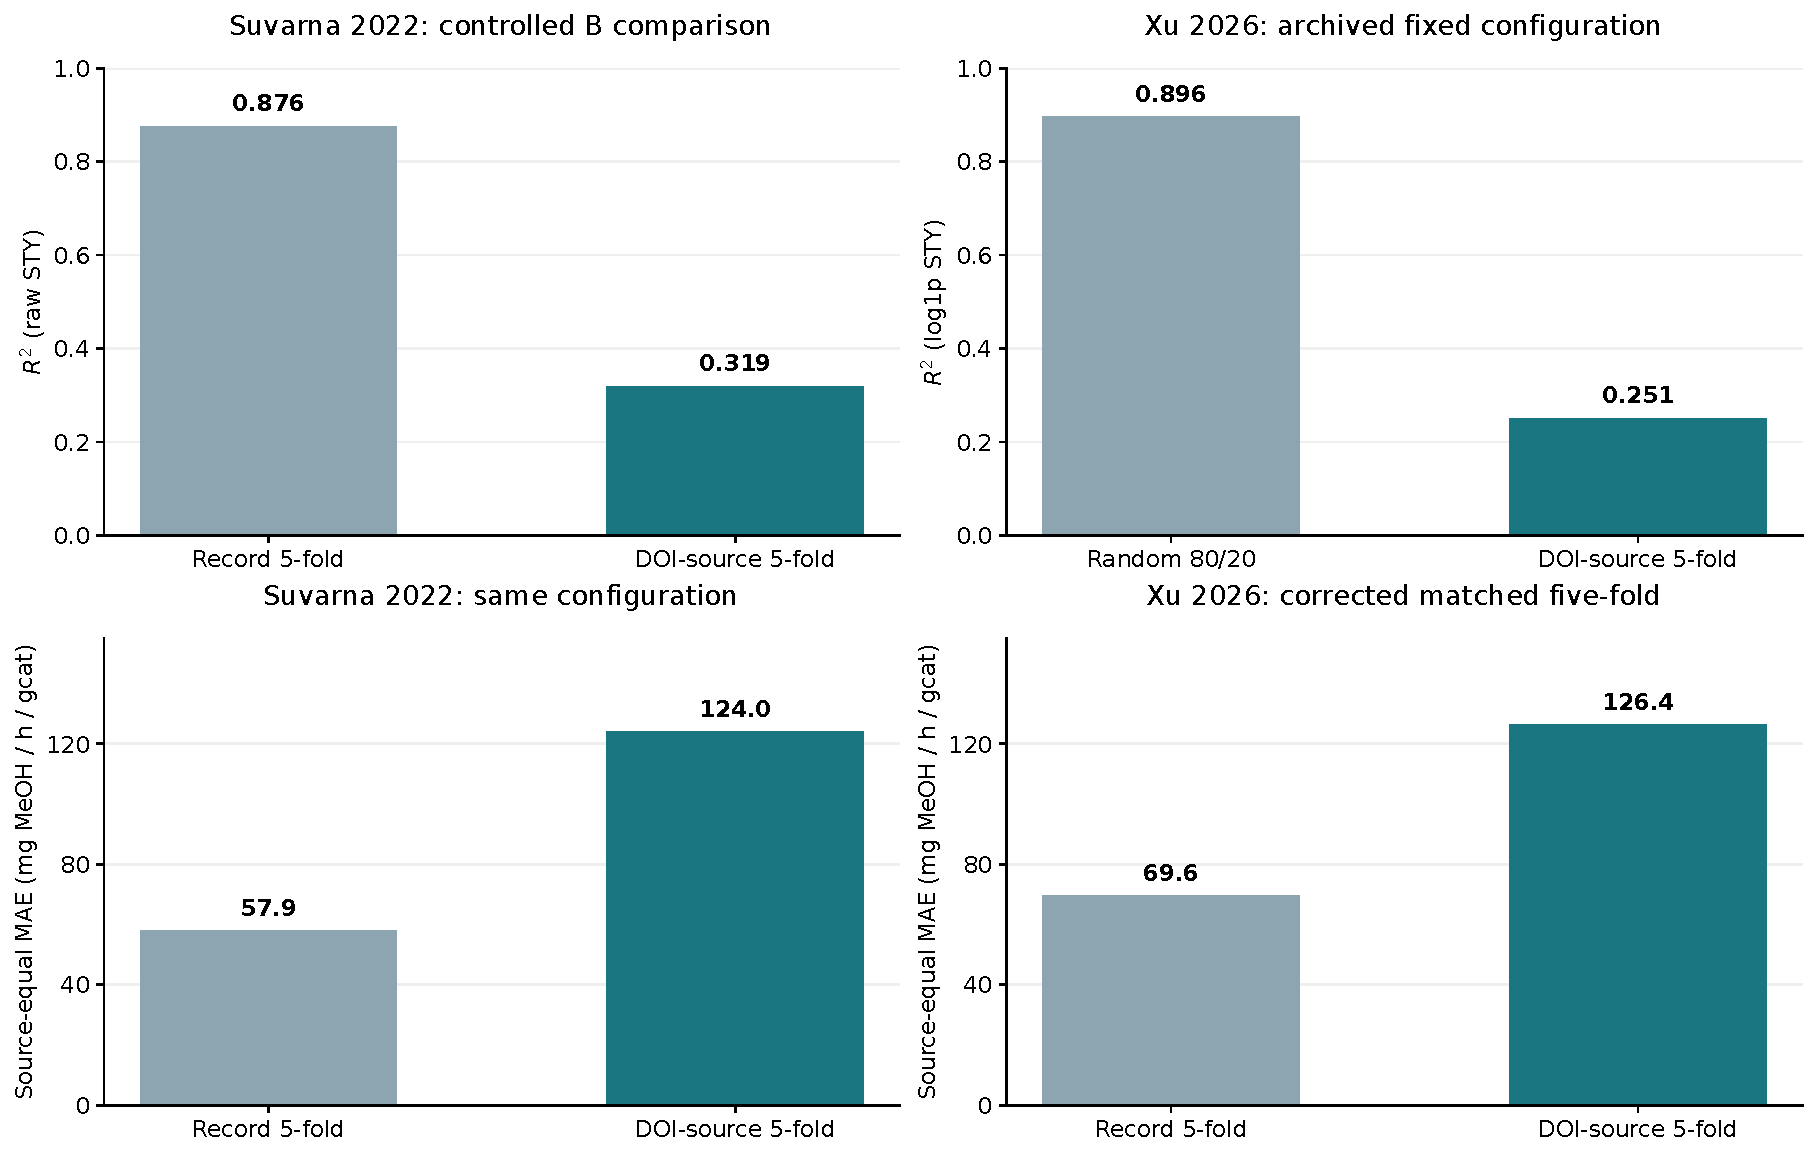
\includegraphics[width=\linewidth]{figs/fig7_published_audit.pdf}
\caption{Published-study audits. Top retains archived $R^2$: Suvarna uses matched five folds; Xu explicitly distinguishes fixed-configuration random 80/20 from source five-fold evaluation. Bottom uses matched-five-fold source-equal MAE, with the corrected source/seed-first Xu aggregation. Author-flow A results are reported separately in the table and are not subtracted across analysis layers.}
\label{fig:audit}
\end{figure}

\paragraph{Author-flow validity and unseen-source interpretation.}
Both studies' author-flow results can be recovered under their own protocols. Predictive scope under source isolation is assessed separately using matched comparisons:
Suvarna's native-STY five-fold $R^2$ changes from 0.876 to 0.319 and source-equal MAE from 57.9 to 124.0;
the later same-five-fold/same-seed Xu audit gives corrected source/seed-first MAE 69.6198 versus 126.3649.
Archived $R^2$ values under different split protocols retain their labels; author-flow A is not subtracted from other analysis layers.
Explaining between-study variance does not replace unseen-publication predictive validation.

\section{Discussion}
\paragraph{From a generalization gap to actionable adaptation.}
Source-disjoint evaluation separates corpus interpolation from prediction for a new publication and determines which gap few-label recovery addresses.
The original budget curves and additional-source application support an actionable positive finding: a small number of new-source measurements can reduce error on the remaining queries given historical data.
Strong local controls and equal-budget design show that measurements reveal response level, conditional relations and useful query coverage.
These are conditional prediction improvements given target support labels; they do not require simultaneous improvement of arbitrary-future-source zero-label accuracy.

\paragraph{Representation supports prediction and measurement allocation.}
The original OCM F0/F1 and Suvarna F5/F17 comparisons establish the need to compare richer descriptors on identical records and splits.
The acquisition--prediction crossing adds another information path: chemistry can guide measurements without entering the deployed predictor.
Equal-budget gains for STY and OCM F1, and improvement in nineteen of twenty within-family identity partitions, directly support this use.
Coverage needs can change with the query population and predictor, so a ranking on one support/query task is not a universal ordering.

\paragraph{Framework contribution and published-study audits.}
Ridge regression, residual calibration, blending, kernel regression and V-optimal design are established tools.
The contribution is a checkable catalysis evidence chain joining source isolation, label budgets, strong local controls, information interventions and representation crossing.
The original two published-study audits remain a distinct final question: author-flow reproduction is separated from controlled split contrasts,
preserving the validity of published results under their own protocols while delimiting their interpretation for unseen sources.
Literature-derived catalysis ML should report record-level and source-disjoint evaluation together, retaining same-label local and equal-budget acquisition controls for adaptation.

\section{Limitations}
Sources are publication entries rather than verified laboratories. Physical preparation batches are not recovered across the historical corpus, and reported identifiers in the measured family do not certify independent physical batches.
Deduplicated literature records are budget units, not guaranteed independent experiments. Reporting selection, upstream attribution quality and unaligned GHSV reference states/inert definitions remain relevant.
Composition encoding represents reported fields; missing does not mean absent. Publication non-overlap does not exclude shared laboratories.
The measured application is one family and repeated partitions are not independent external replications. The historical OCM high-temperature stress population has only five eligible sources.
Bootstrap intervals condition on the fitted pipeline and omit full training uncertainty; development comparisons retain their original inferential status.
The two retrospective published-study audits do not estimate prevalence across catalysis ML; Suvarna is a close rather than exact reproduction.
Working covariances and radii are not certified real-response risks. All evidence is retrospective computation on existing measurements, with no new wet experiment or prospective autonomous discovery campaign.

\section{Conclusion}
Source-disjoint evaluation substantially changes the interpretation of performance in literature-derived catalysis ML.
Few new-source labels recover part of the unseen-source error through identifiable response-level, correspondence and coverage information.
Richer representation can support both local conditional fitting and measurement allocation.
At the same five-label budget and frozen predictor, acquisition reduces STY and OCM F1 errors by 19.7\% and 12.1\%, respectively.
Additional publications and measured-family analyses extend the evidence while retaining query-task and independent-source distinctions.
The two published-study audits continue to show that record-level performance does not automatically estimate unseen-source generalization.
The resulting source-aware, budget-matched evidence chain supports reproducible use of limited measurements, adaptation and experimental allocation.

\section*{Data and code availability}
The computational archive retains original and extended analysis tables, provenance, splits, predictions, frozen fits, settings and published-workflow audit records. Supplement A covers the core protocol and Supplement B the complete extensions. Underlying measurements remain attributed to their original data sources and reuse terms. No new wet-laboratory measurements are reported. Public repository identifiers will be supplied through the journal deposit process; no repository DOI is claimed here.

\section*{Reproducibility statement}
The core benchmark, published-workflow reproductions and extensions retain separate environment records, frozen inputs, source/leakage-group splits, model settings, support orders and result tables.
Numerical claims are read from the corresponding archived analysis layer.
The later fixed-RBF extension retains 2,737,000 independently reconstructed predictions with errors below $10^{-9}$, together with row-loss, support/query separation and population audits.
Prediction and repetition counts do not increase the independent-source population.
The recorded Suvarna compatibility changes and Xu environment-dependent preprocessing difference remain explicit; close/original-flow reproduction is not relabelled as exact reproduction.

\begin{thebibliography}{99}\small
\bibitem{toldy} Toldy, \'A. I. et al. TheMeCat: Dataset of Thermocatalytic Conversion of CO$_2$ to Methanol. \emph{Scientific Data} \textbf{13}, 165 (2026). \url{https://doi.org/10.1038/s41597-025-06482-8}.

\bibitem{yan} Yan, M. et al. A machine learning perspective on three decades of methanol synthesis: research framework and experimental operation insights. \emph{Communications Engineering} \textbf{5}, 162 (2026). \url{https://doi.org/10.1038/s44172-026-00706-4}.

\bibitem{suvarna} Suvarna, M., Ara\'ujo, T. P. \& P\'erez-Ram\'irez, J. A generalized machine learning framework to predict the space-time yield of methanol from thermocatalytic CO$_2$ hydrogenation. \emph{Applied Catalysis B: Environmental} \textbf{315}, 121530 (2022). \url{https://doi.org/10.1016/j.apcatb.2022.121530}.

\bibitem{schmack} Schmack, R. et al. A meta-analysis of catalytic literature data reveals property--performance correlations for the OCM reaction. \emph{Nature Communications} \textbf{10}, 441 (2019). \url{https://doi.org/10.1038/s41467-019-08325-8}.

\bibitem{bendavid} Ben-David, S. et al. A theory of learning from different domains. \emph{Machine Learning} \textbf{79}, 151--175 (2010). \url{https://doi.org/10.1007/s10994-009-5152-4}.

\bibitem{roberts} Roberts, D. R. et al. Cross-validation strategies for data with temporal, spatial, hierarchical, or phylogenetic structure. \emph{Ecography} \textbf{40}, 913--929 (2017). \url{https://doi.org/10.1111/ecog.02881}.

\bibitem{efron} Efron, B. \& Morris, C. Stein's estimation rule and its competitors---an empirical Bayes approach. \emph{Journal of the American Statistical Association} \textbf{68}, 117--130 (1973).

\bibitem{feudale} Feudale, R. N. et al. Transfer of multivariate calibration models: a review. \emph{Chemometrics and Intelligent Laboratory Systems} \textbf{64}, 181--192 (2002). \url{https://doi.org/10.1016/S0169-7439(02)00085-0}.

\bibitem{wu} Wu, W., Yang, M., Cheng, P. \& Wang, Y. Reliable Machine Learning Screening of Adsorption Energies Is Better Assessed with Formula-Grouped Cross-Validation. \emph{Catalysts} \textbf{16}, 742 (2026). \url{https://doi.org/10.3390/catal16080742}.

\bibitem{steyerberg2019} Steyerberg, E.\,W. \emph{Clinical Prediction Models}
(Springer, 2019).

\bibitem{mine} Mine, S. et al. Analysis of Updated Literature Data up to 2019 on the Oxidative Coupling of Methane Using an Extrapolative Machine-Learning Method to Identify Novel Catalysts. \emph{ChemCatChem} \textbf{13}, 3636--3655 (2021). \url{https://doi.org/10.1002/cctc.202100495}. Data: \url{https://github.com/mts-uw/OCM}, commit \texttt{dbf7be5aadb30323f825e8f7d7f6bd3012c99dd2}.

\bibitem{nishimura2023new} S. Nishimura, X. Li, J. Ohyama and K. Takahashi. Leveraging machine learning engineering to uncover insights into heterogeneous catalyst design for oxidative coupling of methane. Catal. Sci. Technol. 13, 4646--4655 (2023). \href{https://doi.org/10.1039/d3cy00596h}{doi:10.1039/d3cy00596h}. Author measurements: \url{https://cads.eng.hokudai.ac.jp/datamanagement/datasources/d84c1e22-ceb9-488a-8d45-4c7cf1c603b5/}.

\bibitem{yubi} K. Yu, J. Bi and V. Tresp. Active learning via transductive experimental design. ICML, 1081--1088 (2006). \href{https://doi.org/10.1145/1143844.1143980}{doi:10.1145/1143844.1143980}.

\bibitem{gorodetsky2016} A. Gorodetsky and Y. Marzouk. Mercer Kernels and Integrated Variance Experimental Design: Connections Between Gaussian Process Regression and Polynomial Approximation. SIAM/ASA J. Uncertain. Quantif. 4, 796--828 (2016). \href{https://doi.org/10.1137/15M1017119}{doi:10.1137/15M1017119}.



\bibitem{xu} Xu, W. H. et al. A natural language processing to causality framework for robust knowledge extraction of CO$_2$ hydrogenation with batch effect control. \emph{npj Computational Materials} \textbf{12}, 191 (2026). \url{https://doi.org/10.1038/s41524-026-02065-2}.


\end{thebibliography}


\end{document}
